\hypertarget{_c_counter_8cpp}{}\section{C\+:/portable\+Dev\+Env\+\_\+2017/workspace2017/\+Blatt2/src/\+C\+Counter.cpp-\/\+Dateireferenz}
\label{_c_counter_8cpp}\index{C\+:/portable\+Dev\+Env\+\_\+2017/workspace2017/\+Blatt2/src/\+C\+Counter.\+cpp@{C\+:/portable\+Dev\+Env\+\_\+2017/workspace2017/\+Blatt2/src/\+C\+Counter.\+cpp}}


Definitionen der Klasse \hyperlink{class_c_counter}{C\+Counter}.  


{\ttfamily \#include \char`\"{}C\+Counter.\+hpp\char`\"{}}\newline
Include-\/\+Abhängigkeitsdiagramm für C\+Counter.\+cpp\+:
\nopagebreak
\begin{figure}[H]
\begin{center}
\leavevmode
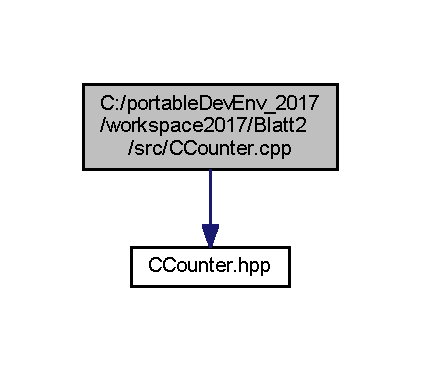
\includegraphics[width=202pt]{_c_counter_8cpp__incl}
\end{center}
\end{figure}


\subsection{Ausführliche Beschreibung}
Definitionen der Klasse \hyperlink{class_c_counter}{C\+Counter}. 

Die bei den Deklarationen in \hyperlink{_c_counter_8hpp}{C\+Counter.\+hpp} genannten Informationen müssen hier nicht mehr wiederholt werden. Dieses File \hyperlink{_c_counter_8cpp}{C\+Counter.\+cpp} bekommen Anwender der Klasse nicht zu Gesicht, daher sind die Kommentare in diesem File als Informationen für Programmierer gedacht, nicht für den Anwender.

Im vorliegenden File werden im wesentlichen die Inhalte der geschweiften Klammern dokumentiert, aber nur dort, wo der Inhalt nicht ohnehin selbsterklärend ist. 